\chapter{概率、泊松过程与散粒噪声}
\label{chap:e03}

\begin{chapteropening}
在导览章（\ref{chap:e00}）里我们已经见到，望远镜最终交给我们的不是一条光滑的电磁波，而是一串离散的点击：某一时刻，某一像素，某一通道，"啪"地记录下一个光子。上一章（\ref{chap:e02}）我们又学会了用带宽和相干时间来刻画这束光作为"波"的一面；可这些波最终是被探测器一颗一颗数下来的。既然是"数"出来的，那就一定有涨落——同样一颗恒星，同样一台望远镜，你连着数十个毫秒，每个毫秒数到的光子数几乎不会相同。这不是仪器坏了，而是"计数"这件事本身自带的呼吸。

本章要把"计数的语言"一次讲透。我们先花几段话把概率论里最少量的几个词（随机变量、期望、方差、独立）复习清楚，然后从"把一段时间切成许多小格"这个极朴素的图像出发，一步不跳地推出泊松分布（Poisson distribution），再由此得到那条贯穿全书的黄金公式：均值等于方差，噪声正比于 $\sqrt{\mu}$。最后我们会问一个更深的问题——如果有一天你测到方差不等于均值，那意味着什么？这个"意味着什么"，正是后面专讲二阶相干 $g^{(2)}$ 的章节要展开的整个故事的入口。
\end{chapteropening}

\section{最小限度的概率复习}
\label{sec:e03-review}

在开始数光子之前，我们需要四个词。它们你在普通物理和概率课上都见过，这里只用"一段话加一个式子"的分量把它们钉牢，方便后面直接调用。

\paragraph{随机变量（random variable）。}
一个随机变量就是"一次实验会给出一个数，但你事先不知道是哪个数"。数一个毫秒里到达的光子数 $N$ 就是最典型的随机变量：它只能取非负整数 $0,1,2,\dots$，而且每个取值都对应一个概率。描述一个（离散）随机变量，就是给出它取每个值的概率 $P(N)$，满足
\begin{equation}
  P(N)\ge 0,\qquad \sum_{N=0}^{\infty}P(N)=1 .
  \label{eq:e03-normalization}
\end{equation}
\begin{formulaexplain}
$N$ 是一次测量得到的整数计数；$P(N)$ 是"这一次恰好数到 $N$ 个"的概率。第一式说概率非负，第二式说把所有可能情况的概率加起来必须是 $1$——总得发生点什么。
\end{formulaexplain}
这里 $N$ 是无量纲的整数（就是"几个"），$P(N)$ 也是无量纲的纯数，取值在 $0$ 到 $1$ 之间。式 \eqref{eq:e03-normalization} 的第二条叫归一化（normalization），它是后面所有推导都必须自洽满足的"守恒律"：不管我们把分布写成多复杂的样子，把 $N$ 从 $0$ 加到无穷，答案必须回到 $1$。

\paragraph{期望（expectation）。}
期望就是"平均值"，但它是一个理论上的、加权的平均：把每个可能取值 $N$ 乘上它的概率再求和。我们用尖括号 $\langle\cdot\rangle$ 表示求期望，
\begin{equation}
  \langle N\rangle=\sum_{N=0}^{\infty}N\,P(N).
  \label{eq:e03-expectation}
\end{equation}
\begin{formulaexplain}
$\langle N\rangle$ 读作"$N$ 的期望"或"$N$ 的平均"；它把每个可能的计数 $N$ 按其发生概率 $P(N)$ 加权求和。它不是某一次的结果，而是无穷多次重复后的平均归宿。
\end{formulaexplain}
注意 $\langle N\rangle$ 一般不是整数——平均每毫秒 $100.3$ 个光子完全合理，尽管任何一次你只能数到整数。期望是可加的：对任意两个随机变量 $X,Y$，$\langle X+Y\rangle=\langle X\rangle+\langle Y\rangle$，无论它们是否独立。这个"期望永远可加"的性质，稍后在拼装小格时会被反复使用。

\paragraph{方差（variance）。}
光有平均值还不够，我们还要知道"每次结果离平均值有多远"。方差衡量的就是涨落的大小：取偏差 $N-\langle N\rangle$，平方（这样正负偏差都变成正贡献），再求期望，
\begin{equation}
  \operatorname{Var}(N)=\big\langle (N-\langle N\rangle)^2\big\rangle
  =\langle N^2\rangle-\langle N\rangle^2 .
  \label{eq:e03-variance}
\end{equation}
\begin{formulaexplain}
$\operatorname{Var}(N)$ 是方差，度量计数围绕其平均值的散布程度；它等于"平方的平均"减去"平均的平方"。它越大，说明每一次数出来的结果越"飘"。
\end{formulaexplain}
式 \eqref{eq:e03-variance} 的第二个等号是一条恒等式，把定义展开即可：$\langle(N-\langle N\rangle)^2\rangle=\langle N^2-2N\langle N\rangle+\langle N\rangle^2\rangle=\langle N^2\rangle-2\langle N\rangle\langle N\rangle+\langle N\rangle^2=\langle N^2\rangle-\langle N\rangle^2$，这里用到了期望可加以及"常数的期望还是它自己"。方差的量纲是 $N$ 的量纲的平方（这里 $N$ 无量纲，所以方差也无量纲）。它的平方根
\[
  \sigma=\sqrt{\operatorname{Var}(N)}
\]
叫标准差（standard deviation），单位和 $N$ 相同，是我们日常说的"误差棒有多长"。请记住这个直觉：$\sigma$ 才是和 $N$ 可比的"涨落尺度"，方差是它的平方。

\paragraph{独立性（independence）。}
两个随机变量独立，直觉上就是"知道其中一个的结果，对另一个的概率分布毫无帮助"。用式子说，联合概率能分解成各自概率的乘积：$P(X=x,\,Y=y)=P(X=x)\,P(Y=y)$。独立性给我们一件极其好用的礼物——方差可加：
\begin{equation}
  \operatorname{Var}(X+Y)=\operatorname{Var}(X)+\operatorname{Var}(Y)
  \quad(\text{当 }X,Y\text{ 独立}).
  \label{eq:e03-var-additive}
\end{equation}
\begin{formulaexplain}
只有当 $X$ 与 $Y$ 相互独立时，它们之和的方差才等于各自方差之和。这条"独立则方差可加"是后面把许多小格拼成一个大 bin、从而算出散粒噪声的关键杠杆。
\end{formulaexplain}
对比一下：期望的可加性 $\langle X+Y\rangle=\langle X\rangle+\langle Y\rangle$ 是无条件的，而方差的可加性 \eqref{eq:e03-var-additive} 需要独立作为前提。原因藏在交叉项里：$\operatorname{Var}(X+Y)=\operatorname{Var}(X)+\operatorname{Var}(Y)+2\operatorname{Cov}(X,Y)$，其中协方差 $\operatorname{Cov}(X,Y)=\langle XY\rangle-\langle X\rangle\langle Y\rangle$ 度量两者的相关；独立时 $\langle XY\rangle=\langle X\rangle\langle Y\rangle$，协方差归零，方差才干净地相加。请把这句话记牢，因为本章末尾"方差不等于均值意味着什么"的整个悬念，就藏在这个协方差是不是零里。

有了这四个词，我们就可以开始真正地数光子了。

\section{一个时间 bin 里的平均计数}
\label{sec:e03-mean}

回到望远镜前。上一章里，探测器把光变成一串离散点击。现在我们做一件最朴素的事：选一个时间窗口（time bin），宽度记作 $\Delta t$，然后数一数这个窗口里落进了几个光子。

如果这束光的平均光子到达率（arrival rate）是 $R_\gamma$，那么一个 bin 里的平均计数就是率乘以时间：
\begin{equation}
  \mu=R_\gamma\,\Delta t .
  \label{eq:e03-mean-count}
\end{equation}
\begin{formulaexplain}
$\mu$ 是一个时间 bin 内的平均光子数（即 $\langle N\rangle$）；$R_\gamma$ 是平均到达率，单位 $\mathrm{s^{-1}}$；$\Delta t$ 是 bin 宽度，单位 $\mathrm{s}$。二者相乘，秒被消掉，$\mu$ 是无量纲的"平均几个"。
\end{formulaexplain}
让我们把单位和数量级坐实。$R_\gamma$ 的量纲是"每秒几个"，即 $\mathrm{s^{-1}}$；$\Delta t$ 的量纲是秒 $\mathrm{s}$；两者相乘，秒和"每秒"抵消，$\mu$ 就是一个纯数。取一组真实的光学观测数字：一颗中等亮度的恒星、一台米级望远镜、一个窄带通道，探测到的光子率大约 $R_\gamma=10^{5}\,\mathrm{s^{-1}}$；若我们把时间切成 $\Delta t=1\,\mathrm{ms}=10^{-3}\,\mathrm{s}$ 的 bin，则
\[
  \mu=R_\gamma\,\Delta t=10^{5}\,\mathrm{s^{-1}}\times10^{-3}\,\mathrm{s}=100 .
\]
也就是说，平均每个毫秒里落进来大约 $100$ 个光子。

这里"平均"两个字必须掰开揉碎地讲，因为它是本章一切的支点。式 \eqref{eq:e03-mean-count} 绝不是说"每个 $1\,\mathrm{ms}$ 窗口都精确收到 $100$ 个光子"。它说的是：如果你在完全相同的条件下（恒星一样亮、望远镜一样大、效率一样高）取来成千上万个 $1\,\mathrm{ms}$ 窗口，把每个窗口数到的光子数加起来除以窗口个数，这个"实测平均"会趋近 $100$。真实的事件流里，这一个 bin 也许是 $92$，下一个也许是 $107$，再下一个是 $100$——它们围着 $100$ 上下呼吸。$\mu$ 是这场呼吸的中心线，不是任何一次的实测值。

关键在于：即便你把一切外部条件都冻结住，让恒星、大气、望远镜、探测器都纹丝不动，这种呼吸也不会消失。这不是"测不准的仪器噪声"，而是"数离散东西"这个动作本身自带的统计涨落。要理解这份涨落到底服从什么规律、有多大，我们需要给"光子彼此独立地稀疏到达"这句物理直觉配上一套数学，那就是泊松分布。

\section{从二项分布到泊松分布：一步不跳的推导}
\label{sec:e03-poisson}

\paragraph{把 bin 切成许多小格}

我们要回答的问题是：既然平均值是 $\mu$，那么"恰好数到 $N$ 个"的概率 $P(N)$ 到底长什么样？

先立一个物理假设，它是整个泊松图像的灵魂：在给定平均率的前提下，光子彼此独立地、无记忆地到达。所谓"无记忆"是说，前一个光子刚到过，既不会招呼下一个也赶紧来（那是聚束），也不会警告下一个别来（那是反聚束）；每一段极短的时间里出不出现光子，只由这段时间的长短决定，和别处发生了什么无关。这正是上一节"平均"背后最简单的到达模式。本章先假设它成立，把结论算到底；至于它何时会被打破，留到最后一节点题。

有了这个假设，就可以用一个非常具体的图像来算。把宽度为 $\Delta t$ 的时间 bin 均匀切成 $M$ 个很短的小格，每个小格宽度
\[
  \delta t=\frac{\Delta t}{M}.
\]
只要 $M$ 足够大、$\delta t$ 足够短，每个小格里最多只可能有一个光子——两个光子同时挤进同一个极短小格的概率可以忽略。于是每个小格就退化成一次最简单的"抛硬币"：要么点击（出现一个光子），要么没有。一个小格发生点击的概率近似为
\begin{equation}
  p=R_\gamma\,\delta t .
  \label{eq:e03-cell-prob}
\end{equation}
\begin{formulaexplain}
$p$ 是单个小格里出现一次点击的概率；$R_\gamma$ 是到达率；$\delta t$ 是小格宽度。率越高、小格越长，这一格里逮到一个光子的机会越大——但只要 $\delta t$ 够短，$p$ 就是个很小的数。
\end{formulaexplain}
$p$ 是无量纲概率（$\mathrm{s^{-1}}\times\mathrm{s}$ 抵消成纯数）。注意这里有个自洽性检查：所有小格的平均点击数加起来，应当正好是整个 bin 的平均计数。确实，$M$ 个小格、每格平均贡献 $p$，总平均就是
\[
  M\,p=M\cdot R_\gamma\frac{\Delta t}{M}=R_\gamma\,\Delta t=\mu .
\]
这个 $Mp=\mu$ 是我们接下来取极限时唯一要"钉死不动"的量：无论把小格切得多细（$M\to\infty$，$p\to0$），乘积 $Mp$ 始终等于 $\mu$。

\paragraph{先写下二项分布}

现在数光子就变成了一道纯组合题："在 $M$ 个小格里，恰好有 $N$ 个格子发生了点击"的概率是多少？由于各小格相互独立，每一种"指定哪 $N$ 个格子点击、其余 $M-N$ 个格子没点击"的具体情形，概率都是 $p^{N}(1-p)^{M-N}$；而"从 $M$ 个格子里选出哪 $N$ 个点击"共有 $\binom{M}{N}$ 种方式。把方式数乘上每种情形的概率，得到二项分布（binomial distribution）：
\begin{equation}
  P_M(N)=\binom{M}{N}p^{N}(1-p)^{M-N},
  \qquad \binom{M}{N}=\frac{M!}{N!\,(M-N)!}.
  \label{eq:e03-binomial}
\end{equation}
\begin{formulaexplain}
$P_M(N)$ 是把 bin 切成 $M$ 个小格后、恰好 $N$ 格点击的概率。$p^{N}$ 是这 $N$ 格都点击、$(1-p)^{M-N}$ 是其余格都不点击、$\binom{M}{N}$ 是"选哪 $N$ 格"的方案数。三者相乘即得。
\end{formulaexplain}
这条式子还没有近似，它是把小格图像精确翻译成概率。$\binom{M}{N}$ 读作"$M$ 选 $N$"，是二项系数；$N!$（$N$ 的阶乘）是排列数的归一化因子，负责除掉"同样这几格、只是数它们的先后顺序不同"的重复。接下来要做的，就是让小格无限变细：$M\to\infty$、$p\to0$，同时死死摁住 $Mp=\mu$。我们把式 \eqref{eq:e03-binomial} 拆成三块——$\binom{M}{N}$、$p^N$、$(1-p)^{M-N}$——一块一块取极限。

\paragraph{\texorpdfstring{第一步：$\binom{M}{N}p^{N}\to \mu^{N}/N!$}{第一步：二项系数那一项的极限}}

把 $p=\mu/M$ 代进去（这是 $Mp=\mu$ 的改写），先合并二项系数和 $p^N$：
\[
  \binom{M}{N}p^{N}
  =\frac{M!}{N!\,(M-N)!}\left(\frac{\mu}{M}\right)^{N}
  =\frac{1}{N!}\cdot\frac{M!}{(M-N)!}\cdot\frac{\mu^{N}}{M^{N}} .
\]
中间那块 $\dfrac{M!}{(M-N)!}$ 其实就是 $N$ 个连续下降的因子相乘：
\[
  \frac{M!}{(M-N)!}=M(M-1)(M-2)\cdots(M-N+1) .
\]
它一共 $N$ 个因子，每个都近似等于 $M$（因为 $N$ 是固定的有限整数，而 $M$ 要趋于无穷，$M-1,M-2,\dots$ 相对于 $M$ 的差别可以忽略）。更精确地，把它除以 $M^{N}$：
\[
  \frac{M(M-1)\cdots(M-N+1)}{M^{N}}
  =1\cdot\Big(1-\tfrac{1}{M}\Big)\Big(1-\tfrac{2}{M}\Big)\cdots\Big(1-\tfrac{N-1}{M}\Big)
  \xrightarrow[M\to\infty]{}1 .
\]
每个括号在 $M\to\infty$ 时都趋于 $1$，而括号只有固定的 $N-1$ 个，所以整段乘积趋于 $1$。于是第一块的极限干净利落：
\begin{equation}
  \binom{M}{N}p^{N}
  =\frac{\mu^{N}}{N!}\cdot\frac{M(M-1)\cdots(M-N+1)}{M^{N}}
  \xrightarrow[M\to\infty]{}\frac{\mu^{N}}{N!}.
  \label{eq:e03-limit-first}
\end{equation}
\begin{formulaexplain}
把 $p=\mu/M$ 代入后，二项系数与 $p^N$ 合并；分子里 $N$ 个下降因子除以 $M^N$ 后逐个趋于 $1$，只剩下 $\mu^N/N!$。这一步把"选格子的组合数"化成了泊松公式里熟悉的 $\mu^N/N!$。
\end{formulaexplain}

\paragraph{\texorpdfstring{第二步：$(1-p)^{M}\to e^{-\mu}$}{第二步：不点击概率的极限}}

现在处理第三块 $(1-p)^{M-N}$。同样代入 $p=\mu/M$：
\[
  (1-p)^{M-N}=\Big(1-\frac{\mu}{M}\Big)^{M-N}
  =\Big(1-\frac{\mu}{M}\Big)^{M}\cdot\Big(1-\frac{\mu}{M}\Big)^{-N}.
\]
先看第二个因子 $\big(1-\mu/M\big)^{-N}$：指数 $-N$ 是固定的有限数，而底数 $1-\mu/M\to 1$，所以这个因子趋于 $1^{-N}=1$，可以扔掉。真正要紧的是第一个因子 $\big(1-\mu/M\big)^{M}$。这里我们点名调用一个标准极限——它就是自然常数 $e$ 的定义式的一般形式：
\begin{equation}
  \lim_{M\to\infty}\Big(1-\frac{\mu}{M}\Big)^{M}=e^{-\mu}.
  \label{eq:e03-elimit}
\end{equation}
\begin{formulaexplain}
这是一条已知的标准极限（$e$ 的定义式）：$\big(1+x/M\big)^{M}\to e^{x}$，取 $x=-\mu$ 即得 $e^{-\mu}$。它把"许多个小格都没点击"的联合概率，凝聚成一个指数因子。
\end{formulaexplain}
为什么 \eqref{eq:e03-elimit} 成立、而不是一句咒语？我们可以取对数验证一遍，用到对数的泰勒展开（Taylor expansion）$\ln(1+u)=u-\tfrac12u^{2}+\cdots$（当 $u$ 很小）：
\[
  \ln\Big(1-\frac{\mu}{M}\Big)^{M}
  =M\ln\Big(1-\frac{\mu}{M}\Big)
  =M\left(-\frac{\mu}{M}-\frac{\mu^{2}}{2M^{2}}-\cdots\right)
  =-\mu-\frac{\mu^{2}}{2M}-\cdots .
\]
当 $M\to\infty$ 时，除第一项外全部含 $1/M$ 的项都消失，只剩 $-\mu$；再取指数还原，就得到 $e^{-\mu}$。物理上，这个 $e^{-\mu}$ 正是"极多个小格、每个都恰好没有点击"的总概率的凝练：$M$ 个小格，每格不点击的概率是 $1-p$，全都不点击就是 $(1-p)^{M}$，在极限下就成了 $e^{-\mu}$。

\paragraph{合起来：泊松分布}

把两步的极限 \eqref{eq:e03-limit-first} 和 \eqref{eq:e03-elimit} 相乘（第二块里被扔掉的 $\big(1-\mu/M\big)^{-N}\to1$ 已并入），二项分布 \eqref{eq:e03-binomial} 就收敛到泊松分布：
\begin{equation}
  P(N)=\lim_{M\to\infty}P_M(N)
  =e^{-\mu}\,\frac{\mu^{N}}{N!}.
  \label{eq:e03-poisson}
\end{equation}
\begin{formulaexplain}
$P(N)$ 是在平均计数为 $\mu$ 时、一个 bin 里恰好数到 $N$ 个光子的概率。$e^{-\mu}$ 来自"许多小格都没点击"，$\mu^{N}$ 是平均越大越偏向多计数的权重，$N!$ 去掉点击排序的重复。这就是稀疏独立到达的计数律。
\end{formulaexplain}
这条式子里每个部件都有对应的直觉。指数因子 $e^{-\mu}$ 是"背景基调"，代表大量空小格的贡献，$\mu$ 越大它压得越低；$\mu^{N}$ 是"越亮越偏多"的爬升项；$N!$ 是组合归一化，抹平了 $N$ 次点击谁先谁后的无关排序。我们可以顺手做一次归一化自检，用到指数函数的泰勒级数 $\sum_{N=0}^{\infty}\mu^{N}/N!=e^{\mu}$（这是 $e^{\mu}$ 的标准展开）：
\[
  \sum_{N=0}^{\infty}P(N)
  =e^{-\mu}\sum_{N=0}^{\infty}\frac{\mu^{N}}{N!}
  =e^{-\mu}\cdot e^{\mu}=1 .
\]
和式 \eqref{eq:e03-normalization} 要求的一样，总概率回到 $1$，说明我们没有在取极限时丢掉或多算概率。

再顺手验证一下期望，确认这个 $\mu$ 确实就是平均计数（而不是某个碰巧同名的字母）。按定义 \eqref{eq:e03-expectation}，
\[
  \langle N\rangle
  =\sum_{N=0}^{\infty}N\,e^{-\mu}\frac{\mu^{N}}{N!}
  =e^{-\mu}\sum_{N=1}^{\infty}\frac{\mu^{N}}{(N-1)!}
  =e^{-\mu}\,\mu\sum_{N=1}^{\infty}\frac{\mu^{N-1}}{(N-1)!}
  =e^{-\mu}\,\mu\,e^{\mu}=\mu .
\]
第一步把 $N=0$ 项（贡献为零）去掉，从 $N=1$ 起求和；第二步用 $N/N!=1/(N-1)!$ 约掉一个因子；第三步换元令 $k=N-1$，那个求和又是 $e^{\mu}$。结果 $\langle N\rangle=\mu$，圆满。至此泊松分布名副其实：它的平均计数正是 $\mu=R_\gamma\Delta t$。

值得强调一句话，免得读者误会泊松分布是什么"神秘的随机"：它描述的绝不是"毫无缘由的乱"，恰恰相反，它描述的是最规矩、最没脾气的一种到达——没有额外记忆、不互相招呼、不互相回避的一串稀疏独立点击。正因为它这么"标准"，它才成了衡量一切偏离的基准线。

\section{散粒噪声：方差等于均值}
\label{sec:e03-shotnoise}

\paragraph{从小格独立叠加算方差}

分布有了，接下来量涨落。我们要证明泊松计数的方差恰好等于它的均值。最省力、也最有物理味道的算法，还是回到小格图像，用第一节备好的"独立则方差可加"这把杠杆。

给第 $i$ 个小格定义一个指示变量（indicator variable）$X_i$：这一格点击了就 $X_i=1$，没点击就 $X_i=0$。总计数就是所有小格的和，$N=\sum_{i=1}^{M}X_i$。每个 $X_i$ 只取 $0$ 或 $1$，是最简单的伯努利变量，它的均值和方差好算：
\[
  \langle X_i\rangle=1\cdot p+0\cdot(1-p)=p,\qquad
  \langle X_i^{2}\rangle=1^{2}\cdot p+0^{2}\cdot(1-p)=p ,
\]
所以由方差定义 \eqref{eq:e03-variance}，
\[
  \operatorname{Var}(X_i)=\langle X_i^{2}\rangle-\langle X_i\rangle^{2}=p-p^{2}=p(1-p).
\]
现在动用假设：不同小格相互独立，于是方差可加（式 \eqref{eq:e03-var-additive}），把 $M$ 个相同的小格加起来，
\[
  \operatorname{Var}(N)=\sum_{i=1}^{M}\operatorname{Var}(X_i)=M\,p(1-p)=Mp\,(1-p)=\mu\,(1-p).
\]
最后一步用了 $Mp=\mu$。现在取小格无限细的极限 $p=\mu/M\to0$，那个 $(1-p)$ 就趋于 $1$，剩下的正是
\begin{equation}
  \operatorname{Var}(N)=\mu .
  \label{eq:e03-var-equals-mean}
\end{equation}
\begin{formulaexplain}
泊松计数的方差恰好等于它的均值 $\mu$。它来自"$M$ 个独立小格、每格贡献 $p(1-p)$ 的方差"叠加，在细分极限下 $(1-p)\to1$，总方差收敛到 $\mu$。均值与方差相等，是泊松统计的指纹。
\end{formulaexplain}
请体会这条 $\operatorname{Var}(N)=\mu$ 是多么苗条而有力：它说，对独立到达的光子，你不需要额外测什么，只要知道平均计数 $\mu$，就自动知道了涨落的大小。均值和方差不是两个独立的量，而是被"独立到达"这个假设锁死成同一个数。这也解释了它为什么叫散粒噪声（shot noise）——就像雨点砸在铁皮屋顶上，噪声不是屋顶坏了，而是雨点本身一颗一颗离散地到达，颗粒感天然带来涨落。

\paragraph{相对噪声、信噪比与数量级}

有了方差，标准差就是它的平方根：
\begin{equation}
  \sigma=\sqrt{\operatorname{Var}(N)}=\sqrt{\mu}.
  \label{eq:e03-sigma}
\end{equation}
\begin{formulaexplain}
$\sigma$ 是计数的标准差，即误差棒的长度，等于 $\sqrt{\mu}$。绝对涨落随平均计数增大而增大，但增得比平均值慢（只按平方根）。
\end{formulaexplain}
注意 $\sigma=\sqrt{\mu}$ 的量纲和 $N$ 一样，都是"几个"，可以直接当误差棒画在计数上：一个平均 $100$ 计数的 bin，典型涨落约 $\sqrt{100}=10$ 个（见图~\ref{fig:e03-poisson}，那条围绕 $\mu$ 铺开的分布和 $\pm\sqrt{\mu}$ 的涨落带就是这套统计的样貌）。绝对涨落确实随亮度上升，但真正决定测量好坏的是它相对于信号本身有多大。于是定义相对散粒噪声（relative shot noise）
\begin{equation}
  \frac{\sigma}{\mu}=\frac{\sqrt{\mu}}{\mu}=\frac{1}{\sqrt{\mu}} .
  \label{eq:e03-relative}
\end{equation}
\begin{formulaexplain}
相对涨落等于 $1/\sqrt{\mu}$：数得越多，相对噪声越小，但只按平方根慢慢改善。想把相对误差压到一半，得多数四倍的光子。
\end{formulaexplain}
这条 $1/\sqrt{\mu}$ 是天文观测里最常被念叨的一句话，把它翻成数量级就格外解渴。它的倒数，$\mu$ 对上它自己的涨落，正是信噪比（signal-to-noise ratio，SNR）：
\begin{equation}
  \mathrm{SNR}=\frac{\text{信号}}{\text{噪声}}=\frac{\mu}{\sigma}=\frac{\mu}{\sqrt{\mu}}=\sqrt{\mu}.
  \label{eq:e03-snr}
\end{equation}
\begin{formulaexplain}
在纯散粒噪声主导时，信噪比就等于 $\sqrt{\mu}$：把信号 $\mu$ 除以它的涨落 $\sqrt{\mu}$。攒到的光子越多，信噪比越高，同样按平方根增长。
\end{formulaexplain}
把真实数字代进去，感受一下这条平方根律有多"贵"。若一段积分下来平均攒到 $\mu=10^{4}$ 个光子，则相对噪声 $1/\sqrt{10^4}=1/100=1\%$，信噪比 $\sqrt{10^4}=100$——这是一次相当漂亮的测量。反过来，若在极暗的源、极短的 bin 里平均只有 $\mu=1$ 个光子，则相对噪声 $1/\sqrt{1}=100\%$，信噪比只有 $1$：此时离散计数本身就是主导噪声，你数到 $0$ 还是 $2$ 几乎是抛硬币，任何精细的物理量都淹没在"有没有光子"的原始涨落里。

这条平方根律也顺带解释了天文观测里那种"事倍功半"的宿命感：想把相对误差从 $1\%$ 再压到 $0.5\%$，$\mu$ 得从 $10^4$ 涨到 $4\times10^4$——积分时间要翻两番，才换来误差减半。散粒噪声是所有更复杂误差预算的地板，后面无论加进背景、死时间还是源自身的变化，都要先站在这块 $\sqrt{\mu}$ 的地板上往上垒。

\begin{figure}[tbp]
\centering
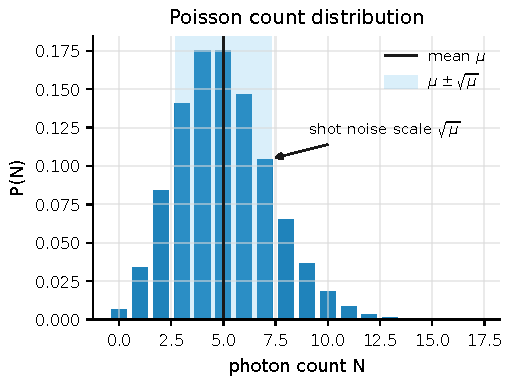
\includegraphics[width=0.85\linewidth]{figures/generated/chapter_01/ch01_photon_count_statistics.pdf}
\caption{泊松计数分布的基本形状（此处取单一平均计数 $\mu$ 作示意）。平均计数为 $\mu$ 时，分布围绕 $\mu$ 铺开，方差也等于 $\mu$，因此涨落的尺度（误差棒）是 $\sqrt{\mu}$，相对散粒噪声为 $1/\sqrt{\mu}$。图中标出了均值线与 $\pm\sqrt{\mu}$ 的涨落带。}
\label{fig:e03-poisson}
\end{figure}

\section{当方差不再等于均值：一个留给后文的问题}
\label{sec:e03-beyond}

现在把整章的逻辑倒过来看一遍。我们得到 $\operatorname{Var}(N)=\mu$，靠的是一个很硬的前提——不同小格里的到达相互独立，从而方差可加（式 \eqref{eq:e03-var-additive}）。这个前提一旦成立，均值和方差就被锁成同一个数。那么反过来：如果有一天你在实验里认认真真地测出方差和均值，发现它们并不相等，这条链子必然是在"独立"这一环断了。

于是"方差比均值大还是小"就成了一个直接读取光子行为的探针。定义一个方便的比值——曼德尔 Q 参数（Mandel $Q$ parameter）——来量化偏离：
\begin{equation}
  Q=\frac{\operatorname{Var}(N)-\mu}{\mu}.
  \label{eq:e03-mandelQ}
\end{equation}
\begin{formulaexplain}
$Q$ 度量计数统计相对泊松的偏离：$Q=0$ 是泊松（独立到达）；$Q>0$ 方差超出均值，称超泊松；$Q<0$ 方差小于均值，称亚泊松。它把"独立不独立"翻成一个可测的数。
\end{formulaexplain}
三种情形对应三幅截然不同的物理画面。$Q=0$，方差等于均值，就是本章的泊松基准，光子彼此不打招呼。$Q>0$，方差鼓出来了，叫超泊松（super-Poissonian）：光子倾向于扎堆到达，一个来了、同伴也更容易结伴而至，仿佛它们爱抱团——这就是聚束（bunching），是热光、星光这类混沌光（chaotic light）的招牌。$Q<0$，方差被压下去了，叫亚泊松（sub-Poissonian）：光子彼此推开，一个刚到、下一个偏偏躲着不来，到达比随机还要"均匀"——这就是反聚束（antibunching），是单光子源等真正非经典光的指纹，经典电磁波无论如何摆弄都做不出来。

把这两幅画面推到极端，就触到本章末尾埋下的那个协方差：聚束意味着相邻时间的到达是正相关的（$\operatorname{Cov}>0$，方差被顶大），反聚束意味着负相关（$\operatorname{Cov}<0$，方差被削小）。度量这种"一个光子到达之后、另一个光子更可能还是更不可能紧跟着到达"的相关强度，需要一个专门的工具——二阶相干函数（second-order coherence）$g^{(2)}(\tau)$。它测的正是"在时刻 $t$ 探测到一个光子的条件下，再过 $\tau$ 又探测到一个光子"的相对概率：$g^{(2)}(0)>1$ 是聚束，$g^{(2)}(0)<1$ 是反聚束，$g^{(2)}=1$ 回到本章这条各处独立的泊松基线。

换句话说，本章把"计数的语言"讲到了它的边界：只要光子独立到达，一切都被 $\mu=R_\gamma\Delta t$ 和 $\operatorname{Var}(N)=\mu$ 两条式子锁定。而真正有趣的天体物理和量子光学，恰恰住在这条边界之外——住在方差偏离均值、光子开始互相"感知"彼此的地方。如何系统地度量这份偏离、它又如何反过来告诉我们光源的物理性质乃至天体的角尺度，是后面专讲二阶相干 $g^{(2)}$ 的章节要展开的正题。到那时你会看到，本章这条不起眼的 $\operatorname{Var}(N)=\mu$，正是整座强度干涉大厦的地基。

\section{本章要点}
\label{sec:e03-summary}

\begin{itemize}
  \item \textbf{四个词。}随机变量给出取每个值的概率（归一化 $\sum P(N)=1$）；期望 $\langle N\rangle$ 永远可加；方差 $\operatorname{Var}(N)=\langle N^2\rangle-\langle N\rangle^2$ 度量涨落；独立性让方差也可加——这是全章最关键的杠杆。
  \item \textbf{平均计数。}一个时间 bin 的平均计数 $\mu=R_\gamma\Delta t$；取 $R_\gamma=10^5\,\mathrm{s^{-1}}$、$\Delta t=1\,\mathrm{ms}$ 得 $\mu=100$。"平均"是许多同条件 bin 的归宿，不是任何一次的实测值。
  \item \textbf{泊松分布。}把 bin 切成 $M$ 个小格、每格点击概率 $p=\mu/M$，计数服从二项分布 \eqref{eq:e03-binomial}；令 $M\to\infty$，用 $\binom{M}{N}p^N\to\mu^N/N!$ 和标准极限 $(1-\mu/M)^M\to e^{-\mu}$，得 $P(N)=e^{-\mu}\mu^N/N!$。
  \item \textbf{散粒噪声。}由小格独立叠加得 $\operatorname{Var}(N)=\mu$；标准差 $\sqrt{\mu}$，相对散粒噪声 $1/\sqrt{\mu}$，信噪比 $\sqrt{\mu}$。$\mu=10^4$ 时相对误差 $1\%$；$\mu=1$ 时计数本身主导。误差减半要多数四倍的光子。
  \item \textbf{边界之外。}方差偏离均值（$Q\neq0$）意味着光子不再独立到达：超泊松对应聚束，亚泊松对应反聚束。度量这份相关的工具是二阶相干函数 $g^{(2)}$，留待后面专讲它的章节展开。
\end{itemize}

\medskip
\noindent\textbf{想一想。}
\begin{enumerate}
  \item 若把 bin 宽度 $\Delta t$ 加倍，$\mu$、$\sigma$、相对噪声 $1/\sqrt{\mu}$ 各自如何变化？信噪比呢？
  \item 一台望远镜每秒探测 $10^6$ 个光子，你想让某个测量的相对散粒噪声达到 $0.1\%$，至少要积分多久（假设纯散粒噪声）？
  \item 假如你测到某个源的方差明显小于均值（$Q<0$），在完全排除仪器问题后，这在物理上意味着什么？经典电磁波能给出这种结果吗？
\end{enumerate}
